%! TEX root = ../main.tex
% ============================================================
% IMMUTABLE — generated automatically, do not edit this block
%   script          : plotter.py::plot_frequency_spectrum
%   plot_type       : spectrum_fft
%   chapter         : 05
%   panel           : reverse
%   wind            : no, lowest, full
%   amplitude       : 0.1
%   frequency       : 1.3
%   probes          : 2, 3
%   data_type       : fft
%
% PANELS AVAILABLE:
%   FIGURES/05_spectrum_fft_reversepanel-no-lowest-fullwind-amp0100-freq1300-probe2.pdf
%   FIGURES/05_spectrum_fft_reversepanel-no-lowest-fullwind-amp0100-freq1300-probe3.pdf
% ============================================================
\begin{figure}[htbp]
  \centering
  \begin{subfigure}[b]{0.48\linewidth}
    \centering
    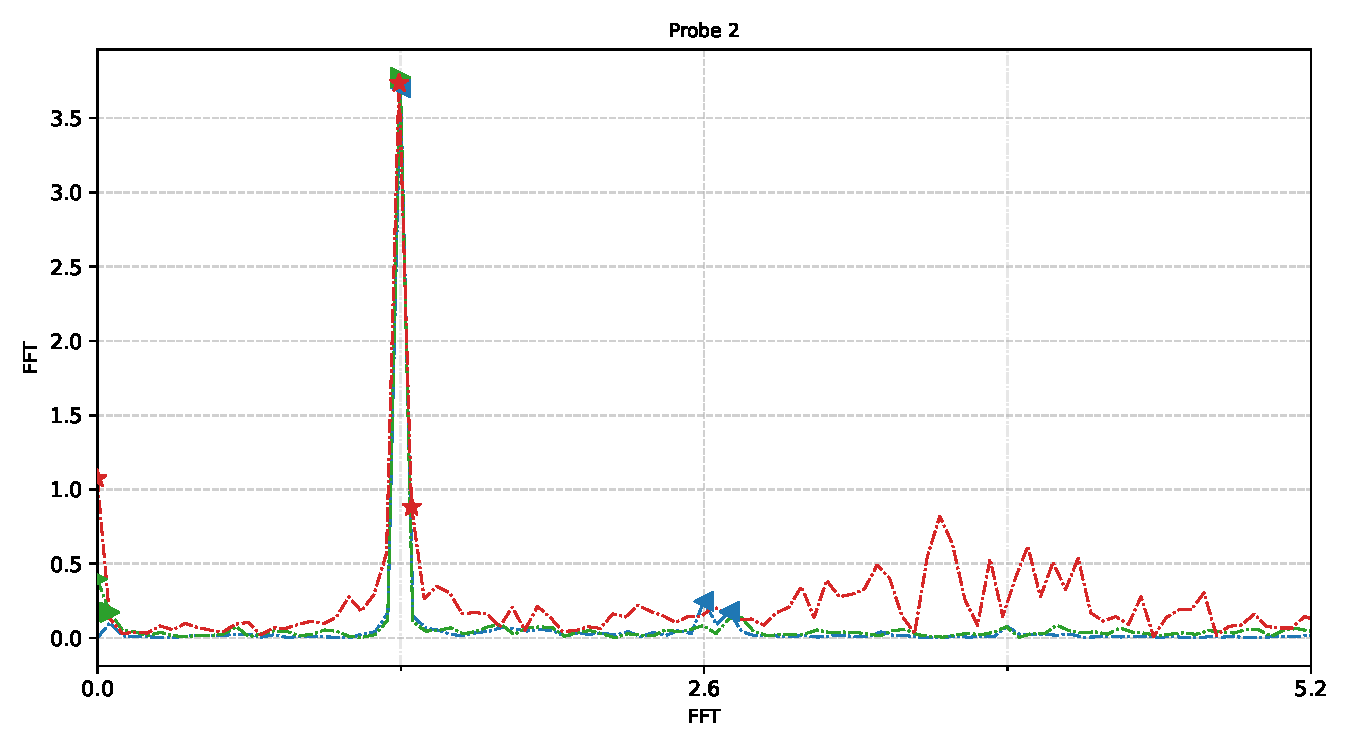
\includegraphics[width=\linewidth]{FIGURES/05_spectrum_fft_reversepanel-no-lowest-fullwind-amp0100-freq1300-probe2.pdf}
    \caption{TODO}
    \label{fig:TODO_2}
  \end{subfigure}
  \hfill
  \begin{subfigure}[b]{0.48\linewidth}
    \centering
    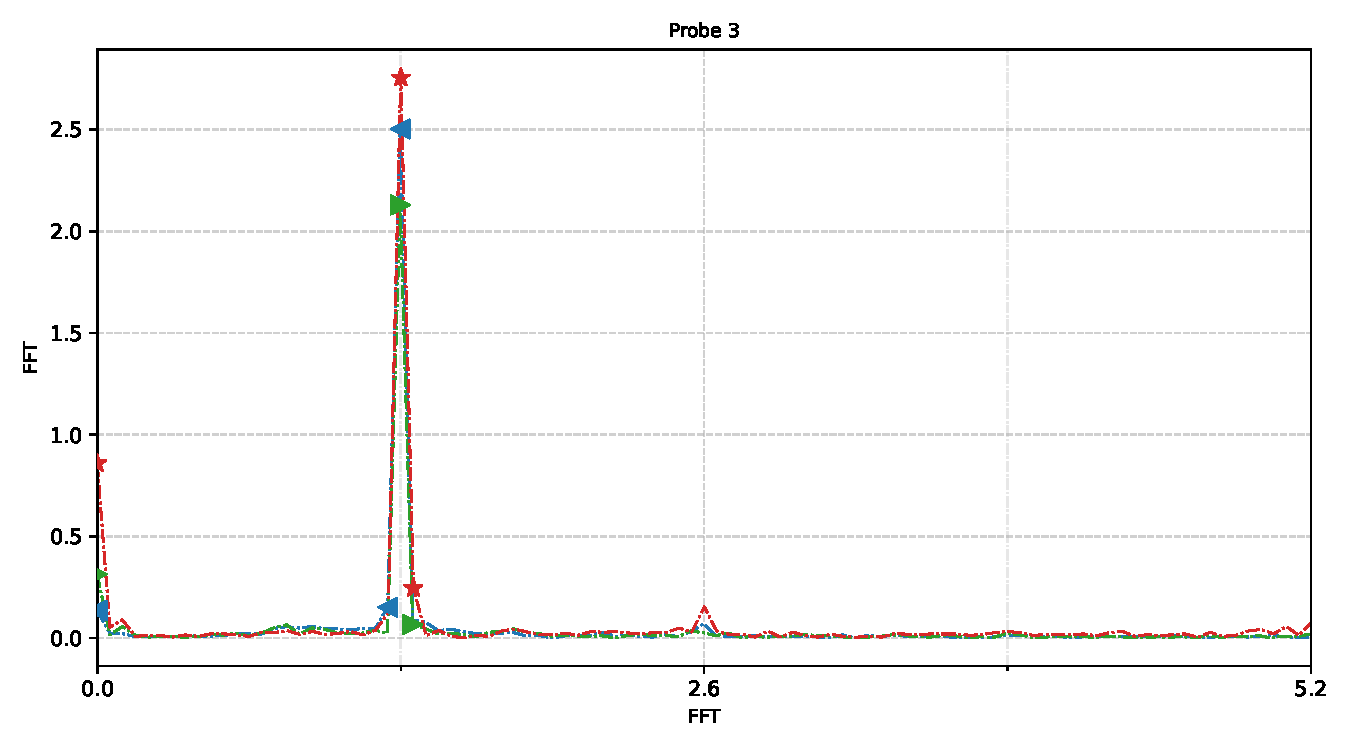
\includegraphics[width=\linewidth]{FIGURES/05_spectrum_fft_reversepanel-no-lowest-fullwind-amp0100-freq1300-probe3.pdf}
    \caption{TODO}
    \label{fig:TODO_3}
  \end{subfigure}
  \caption[Short caption for LOF]{
    % TODO: write caption
  }
  \label{fig:TODO_ind-amp0100-freq1300-probe2og3}
\end{figure}
